The demand for clean and firm energy has increased, while the world grapples
with the effects of climate change. Many utilities and decision-makers have
been increasingly faced with the rising energy demands of machine learning and
data center companies, which require a constant and reliable energy source, on
top of existing demands from our increasingly electrified lives. The emergence
of data center demand has led the \gls{eia} to forego publishing their annual
energy outlook in 2023 as they focus on incorporating emergent market pressures
\cite{eia_annual_outlook_canceled_2023}. To meet these demands, companies and
utilities are looking to new nuclear reactors that can provide clean, firm
energy. These reactors are designed to be more efficient, flexible, and
resilient than the reactors that have come before them.

Since 1959, the \gls{usa} has commercially operated large \gls{lwr} designs at
nuclear power plants. These reactors use light water as a coolant and moderator
and can be categorized as either \glspl{pwr} or \glspl{bwr}. As shown in Figure
\ref{fig:online_lwr_cap_2024}, the \gls{lwr} fleet in the \gls{usa} expanded
capacity over a period of roughly 20 years before achieving just over 99 GWe in
1990 and remained roughly constant in the years since then. With the recent
connection of Vogtle Units 3 and 4 to the grid, the \gls{usa} has seen the
first new \gls{lwr} units come online in 8 years--following the completion of
Watts Bar-2 in 2016.

\begin{figure}[H]
    \centering
    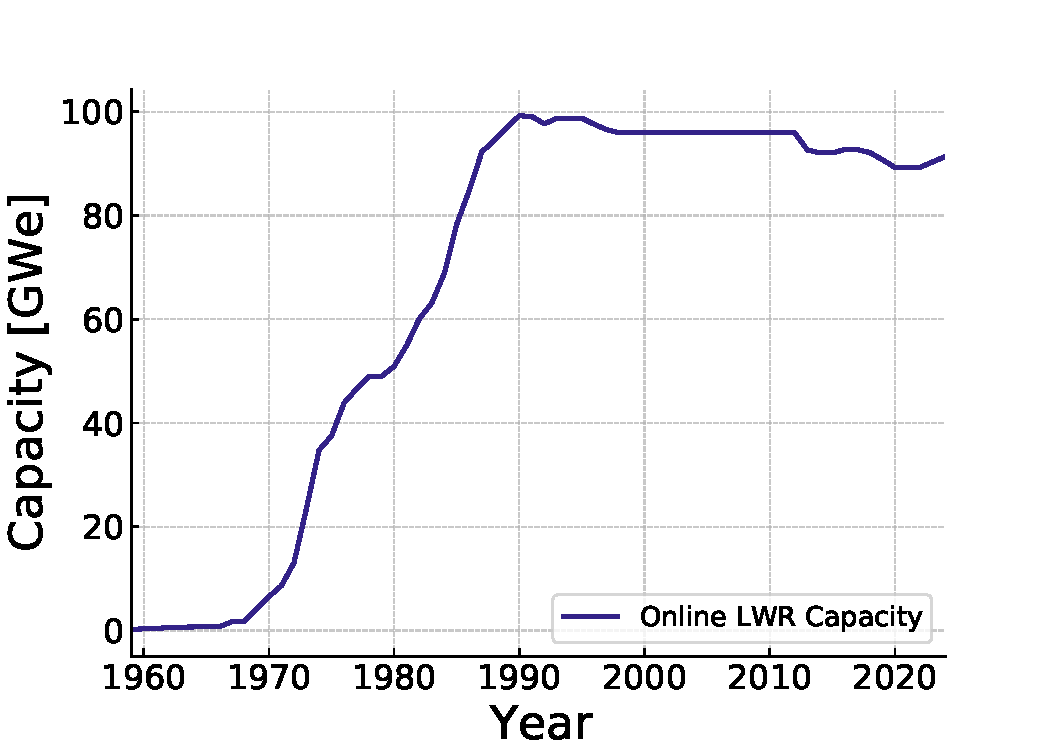
\includegraphics[scale=0.7]{images/intro/online_lwr_cap_2024.pdf}
    \caption{US LWR Capacity through 2024 \cite{IAEA_PRIS}}
    \label{fig:online_lwr_cap_2024}
\end{figure}

According to the \gls{eia}, nuclear energy made up 18\% of utility-scale
electricity generation in 2023 \cite{eia_elec_gen_2024}, which makes it 46.5\%
of total clean energy generation and the largest producer of clean energy in
the country. The last license in the fleet will now expire in 2063 following
the completion of Vogtle Unit 4, but, to meet our growing energy demands the
\gls{usa} will need to replace and expand the current fleet as it retires over
that time; deploying new reactors at a rate that has not been seen since the
1970s. The \gls{doe} has published a liftoff report on the potential for
nuclear energy to meet the demands of the future, and has outlined a variety of
scenarios that could lead to a 100\% clean energy future by 2050
\cite{julie_liftoff_pathways_2024}. One of the striking takeaways from the
liftoff report is the potential demand for nuclear to triple by 2050 due to new
capacity demand, the retirement of fossil fuels, electrification of our
economy, and other behind-the-meter applications of nuclear technologies. The
potential that \gls{doe} outlines is not without its challenges; the \gls{eia}
2023 Domestic Uranium Production Report highlights the decrease in uranium
concentrate production in the \gls{usa} and the number of fuel cycle facilities
that are dormant or have been decommissioned \cite{eia_uranium_statistics_2023}.

Despite these deployment challenges, the \gls{doe} liftoff report asserts that
high-value propositions in low land use, firm energy generation, direct heat
applications, local economic benefits, and the low transmission build-out
associated with nuclear energy make it a compelling choice. Some of these
benefits can be reflected in the 73\% increase in uranium production workers
from 2022 to 2023, the 4x increase in exploration of uranium resources, and
\$20 million increase in resource investment \cite{eia_uranium_statistics_2023}
--the private sector is starting to move on nuclear's value proposition.

The current fleet of \glspl{lwr} has been the backbone of the commercial nuclear
industry, but the industry is on the precipice of a different generation of
reactor technologies. The fleet of \glspl{lwr} uses a ceramic uranium-oxide fuel
that is enriched to 3-5\% $^{235}$U, but there is a panoply of advanced reactor
designs that are at various stages of deployment making use of our decades of
experience with nuclear energy. These reactors vary in size from large
gigawatt-scale reactors to smaller reactors that can fit on the back of a
truck. The design space is vast, but one innovation that has been a focus of
the nuclear industry is the \gls{triso} fuel particle. This fuel particle is a
small sphere of uranium fuel that is coated in layers of carbon and silicon
carbide. \gls{triso} is designed to be more robust than traditional fuel and
can be used in a variety of reactor designs that require higher enrichments of
$^{235}$U, into \gls{haleu} territory (5-20\%).

The \gls{nfc} describes the plethora of steps nuclear fuel goes through
in its life cycle. In Figure \ref{fig:once-through} we have outlined a
simple "once-through" fuel cycle (so-called because the fuel goes through
the cycle once in its lifetime). The fuel cycle begins with mining uranium ore,
typically from uraninite or pitchblende deposits. Then the ore must be milled
and refined into yellowcake, which can then be converted into uranium
hexafluoride. To power the reactors in the \gls{usa}, the uranium hexafluoride
is then enriched to the desired percentage of $^{235}$U, and then converted
into uranium dioxide. Reactor operators receive the fuel in rods after it has
been fabricated into fuel pellets from uranium dioxide. Upon receiving the
fuel, workers load the rods into the reactor to generate heat. The heat
generates steam, which drives a turbine and generates electricity. After years
of operation, workers remove the used fuel from the reactor and store it in a
spent fuel pool. After a period of cooling time, transporters move the used
fuel to dry cask storage, where it will remain until policymakers act to enable
a long-term solution.

\begin{figure}[H]
    \centering
    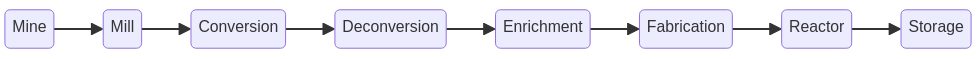
\includegraphics[scale=0.40]{images/once_through_fc.png}
    \caption{US Once-through Fuel Cycle}
    \label{fig:once-through}
\end{figure}

Although we have linearly presented them, these steps are interwoven with
multilateral relationships, and long-term purchasing agreements that complicate
the establishment of new supply chains. As a consequence, the availability of
services at each step in the fuel cycle is difficult to model; this is where we
make use of the \cyclus \cite{huff_cyclus_intro_2016} tool. \cyclus is a
nuclear fuel cycle simulator that allows users to model the movement of
material between facilities in discrete-event simulations. These facilities
are run by agents that make decisions and interact with other agents. Because
\cyclus is designed to be technology agnostic, we can use it to model a variety
of fuel cycles and reactor types--although it is not primarily a physics code,
and coupling it with true physics codes can be necessary for some problems.

Partners in industry, academia, and government are building the body of
literature surrounding \gls{triso} fuel cycles. This work is a timely
evaluation of a variety of energy-demand scenarios and an optimization of the
deployment of advanced reactors building off of the method established by
Bachmann et al. \cite{bachmann_enrichment_2021} for \gls{haleu} fuel,
incorporating the staggered enrichment demand that advanced reactor
companies could explore as the \gls{haleu} supply chain
develops. We seek to understand the deployment of advanced reactors in the
\gls{usa} and the implications of the fuel cycle on the deployment of these
reactors as some designs adopt a staggered enrichment demand for a variety of
\gls{triso} fuels. We have chosen to focus on \gls{swu},
energy output, mass of fuel, and reactor deployment to understand
the performance of each deployment scenario. In
service of this goal, we will also examine the computational efficiency of the
\gls{dre} in \cyclus to contribute to a robust tool for future analysis.


The structure of this thesis is as follows:

\begin{itemize}
    \item Chapter 2 outlines energy system modeling, the reactors used in this work, the types of fuel, and the \cyclus tool as it pertains to this work.
    \item Chapter 3 discusses the deployment schemes used in this work, the metrics used to evaluate the scenarios, and presents the results of each.
    \item Chapter 4
    \item Chapter 5 concludes the work in Chapters 3 and 4, discusses the assumptions and limitations, and presents directions for future work.
    \item Appendix A discusses what we call the "existing fleet" in this work.
    \item Appendix B discusses the implemented reactor deployment schemes that were not used in this work.
    \item Appendix C discusses the availability and reproducibility of this work.
\end{itemize}